% !Mode\dots ``TeX:UTF-8''
\documentclass[serif]{beamer}
%\usetheme{Warsaw}
\usepackage{hyperref}
\usepackage{subcaption}
\usepackage{euscript}
%\usepackage{natbib}
\DeclareGraphicsExtensions{.png,.jpg}
\usepackage{default}


%自定义的宏
\include{def}
% 图片路径
\graphicspath{{img/}}
\title{BlockChain}
%\subtitle{network flows problems}
\author{ Liyun Dai}

\institute{RISE, Southwest University, Chongqing, China}
\date{\today}

\begin{document}
\maketitle
\begin{frame}
  \frametitle{Table of Contents}
  \tableofcontents[currentsection]
\end{frame}

\AtBeginSection[]
{\begin{frame}
	\frametitle{Table of Contents}
		\tableofcontents[currentsection]
\end{frame}}
\section{INTRODUCTION}

\begin{frame}{Original problem}
	\begin{problem}
		The original problem comes from the idea to have some
		thing represented as {\color{red}{digital entity}} that can be passed {\color{red}{securely}}
		from one party to another.
	\end{problem}
\end{frame}

\begin{frame}{Example}
	\begin{example}
		Imagine you have some money in
		your bank account, and you would like to securely transfer
		some of it to another person
	\end{example}
	
	{\Huge Bank is a trusting center.}
\end{frame}

\begin{frame}{Example 	without bank }

	\begin{problem}
		Yes it is possible. However, regardless of representation any digital sequence can be copied.
		This creates the well-known problem of {\color{red}{“double-spending”}}:
		one person makes an electronic transaction more than once
		using the same money.
	\end{problem}
\end{frame}
\section{HASH FUNCTIONS}
\begin{frame}{Hash function}
	\begin{definition}
		Hash function is a method to convert data of arbitrary size
		into a digital string of predefined {\color{red}{fixed length}}, called hash.
	\end{definition}
\end{frame}
\begin{frame}{Hash function}
		\begin{definition}[cryptographic hash functions]
			It should be easy to compute the hash, but finding any input to the hash
			function {\color{red}{must be difficult}}, or better virtually impossible. Hash functions with such a property are sometimes called
			cryptographic hash functions.
		\end{definition}
\end{frame}
\begin{frame}{Example}
	The best known cryptographic hash functions are
	{\tt MD5}, {\tt SHA1}, {\tt SHA2}. 
	\begin{example}
		An example of {\tt MD5} is this
		{\tt MD5}(``abc") = 900150983cd24fb0d6963f7d28e17f72
	\end{example}
\end{frame}

\begin{frame}{HASHCHAINS}
		\begin{figure}
		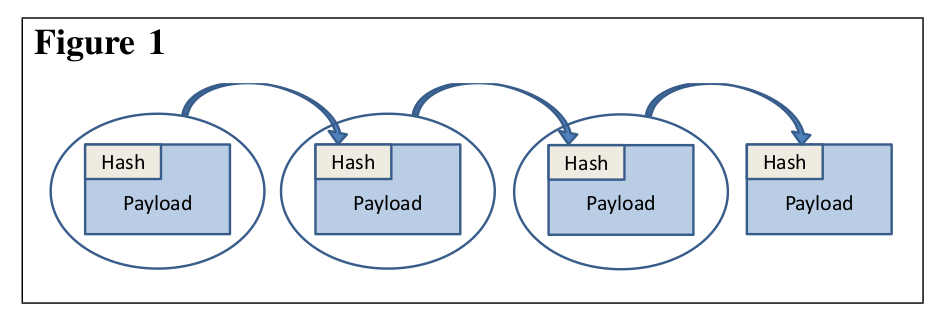
\includegraphics[width=0.8\textwidth]{hashch}
		\label{fig:hash}
	\end{figure}
	\begin{block}{Integrity}
		This hashchain has the important property: no data can be modified at any block
		without affecting the integrity of the subsequent blocks.
	\end{block}
	
	
\end{frame}

\begin{frame}{Add a new block}
	Next step is to authorise only one person to create a
	new block in the chain. One way to do it is {\color{red}{Public Key
	Cryptography}} (PKC).
\end{frame}

\section{PUBLIC KEY CRYPTOGRAPHY}

\begin{frame}{PKC}
	\begin{definition}
			Given some data m (m for message) {\color{red}{anyone}}
			can compute encrypted value Enc(m). But, {\color{red}{only the one}} who
			knows a special key related to this encryption can compute in
			the opposite way, i.e. find m from Enc(m).
	\end{definition}
\end{frame}

\begin{frame}{Two scenarios of PKC}
	\begin{enumerate}[<+->]
		\item The first is when one party wants to send a secure message to another.
		\item Identity certificate.
	\end{enumerate}
\end{frame}

\begin{frame}{Send a secure message to another}
	\begin{figure}
		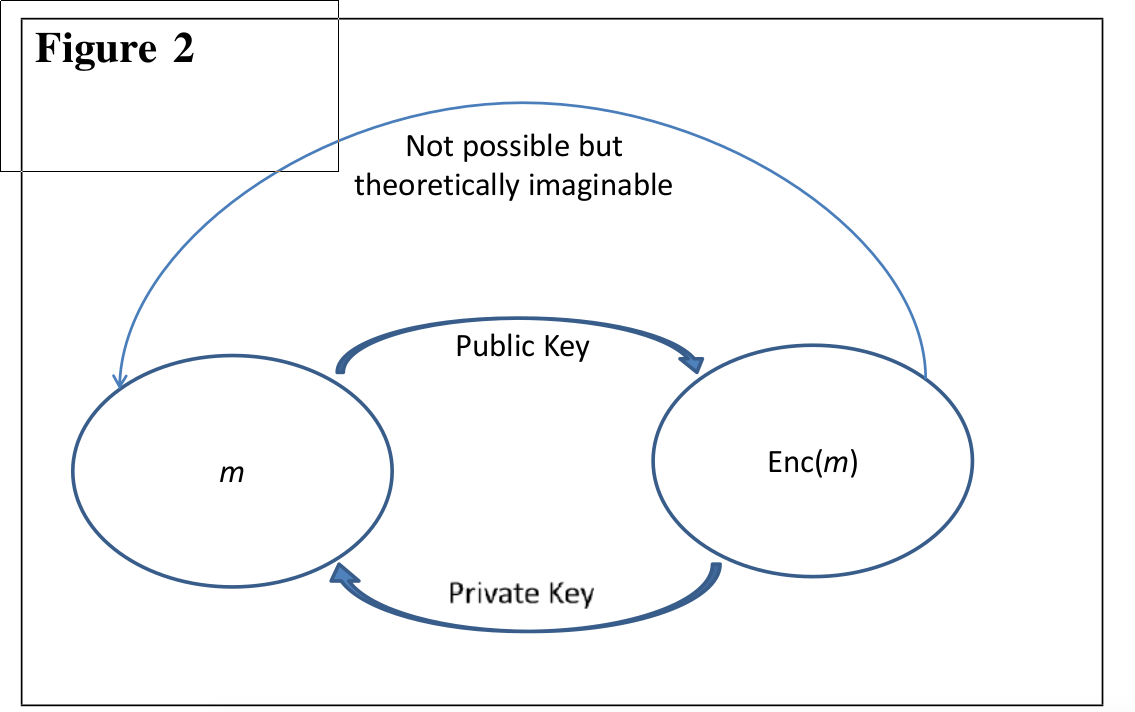
\includegraphics[width=0.7\textwidth]{pkc}
		\label{fig:pkc}
	\end{figure}	
\end{frame}




\section{SECURING HASHCHAIN WITH PUBLIC KEY CRYPTOGRAPHY}

\begin{frame}{Problem}
	\begin{problem}
		Now, let’s go back to the question of whether it is possible
		that only one person is enabled to add a block to the hashchain.
	\end{problem}
\end{frame}

\begin{frame}{Bitcoin}
		\begin{figure}
			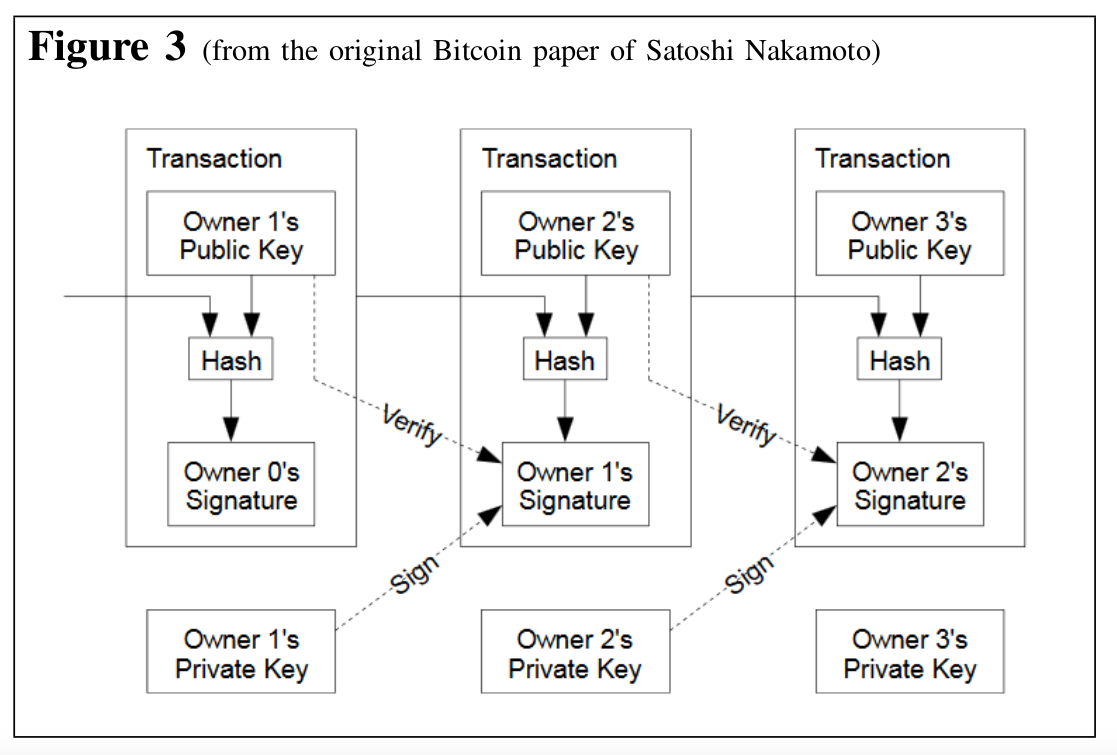
\includegraphics[width=0.7\textwidth]{bit}
			\label{fig:bit}
		\end{figure}
	
\end{frame}


\section{BLOCKCHAINS}
\begin{frame}{BlockChain}
	\begin{figure}
		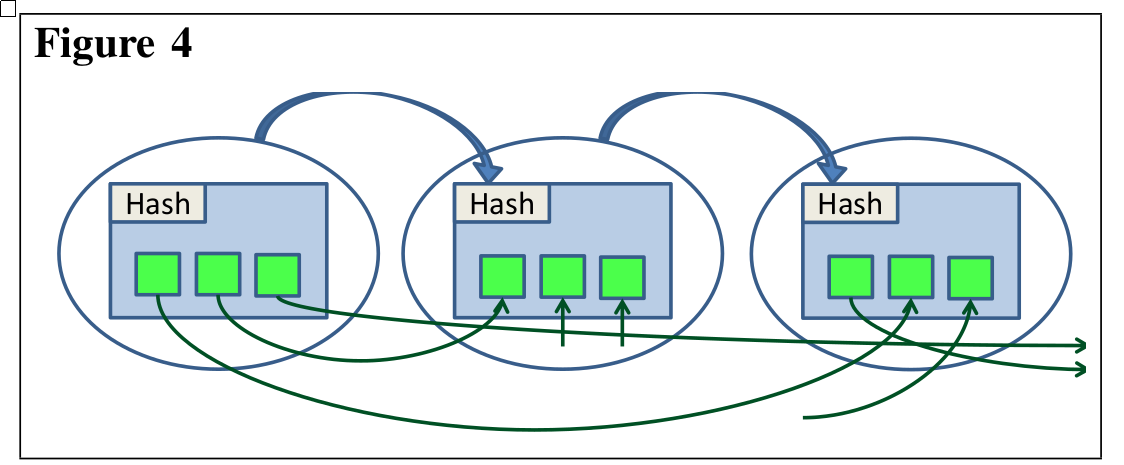
\includegraphics[width=0.7\textwidth]{block}
		\label{fig:block}
	\end{figure}
	
\end{frame}


\begin{frame}{Different types of systems}
	
	\begin{figure}
		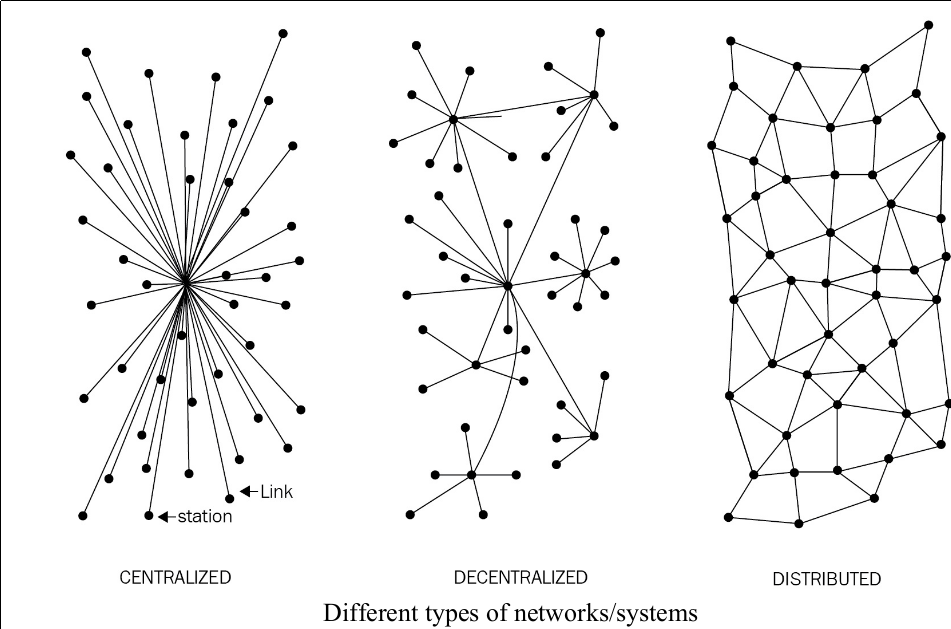
\includegraphics[width=0.7\textwidth]{types}
		\label{fig:4D}
	\end{figure}

\end{frame}



\begin{frame}{Fundamental questions}
 Is a blockchain really needed? When is a blockchain required? In
	what circumstances is blockchain preferred over traditional databases? 
	\begin{enumerate}[<+->]
		\item Is high data throughput required? If the answer to this question is yes, then use a traditional database.
		\item Are updates centrally controlled? If yes, then use a conventional database.
		\item Do users trust each other? If yes, then use a traditional database.
		\item Are users anonymous? If yes, then use a public blockchain; if not, then use a private blockchain.
		\item If consensus is required to be maintained within a consortium then use a private blockchain, otherwise use
		a public blockchain. 
	\end{enumerate}
\end{frame}
\end{document}